% Created 2024-01-30 Tue 14:32
% Intended LaTeX compiler: pdflatex
\documentclass[11pt]{article}
\usepackage[utf8]{inputenc}
\usepackage[T1]{fontenc}
\usepackage{graphicx}
\usepackage{longtable}
\usepackage{wrapfig}
\usepackage{rotating}
\usepackage[normalem]{ulem}
\usepackage{amsmath}
\usepackage{amssymb}
\usepackage{capt-of}
\usepackage{hyperref}
\usepackage{minted}
\usepackage[russian]{babel}
\author{Кормышев Егор}
\date{\today}
\title{CMS}
\hypersetup{
 pdfauthor={Кормышев Егор},
 pdftitle={CMS},
 pdfkeywords={},
 pdfsubject={},
 pdfcreator={Emacs 28.2 (Org mode 9.5.5)}, 
 pdflang={Russian}}
\begin{document}

\maketitle
\tableofcontents


\section{Определение}
\label{sec:orgde84f99}

\textbf{CMS (Content Managment System)} - програмная основа для разработки и редактирования сайта. 

\section{Функции CMS}
\label{sec:orgf21b28e}

\begin{itemize}
\item Создание
\item Управление
\item Публикация
\item Представление
\end{itemize}

\section{Категории CMS}
\label{sec:org95e5d13}

\begin{itemize}
\item системы управления исходными кодами
\item системы управления доккументами
\item системы управления web-контентом
\item системы управления интернет магазинами
\end{itemize}

\section{Виды CMS}
\label{sec:orgb3c0bb6}

\begin{itemize}
\item коробочные
\item самописные
\item headless CMS
\end{itemize}

\section{Архитектура CMS}
\label{sec:org55160fc}
\begin{figure}[htbp]
\centering
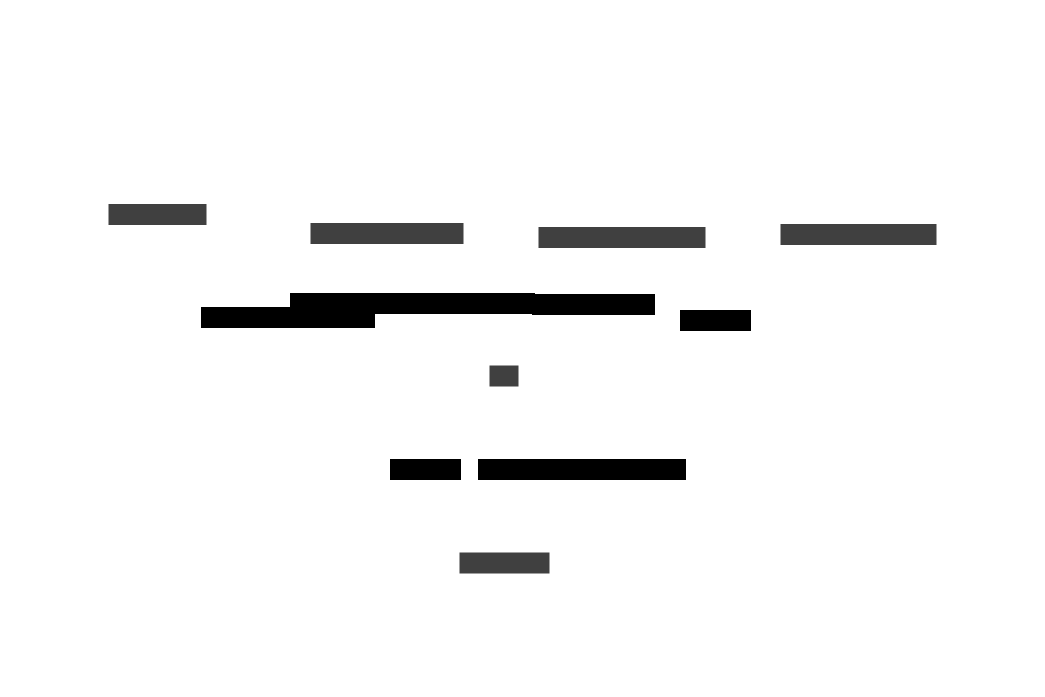
\includegraphics[width=.9\linewidth]{./pic.png}
\caption{схема работы над CMS}
\end{figure}
\begin{figure}[htbp]
\centering
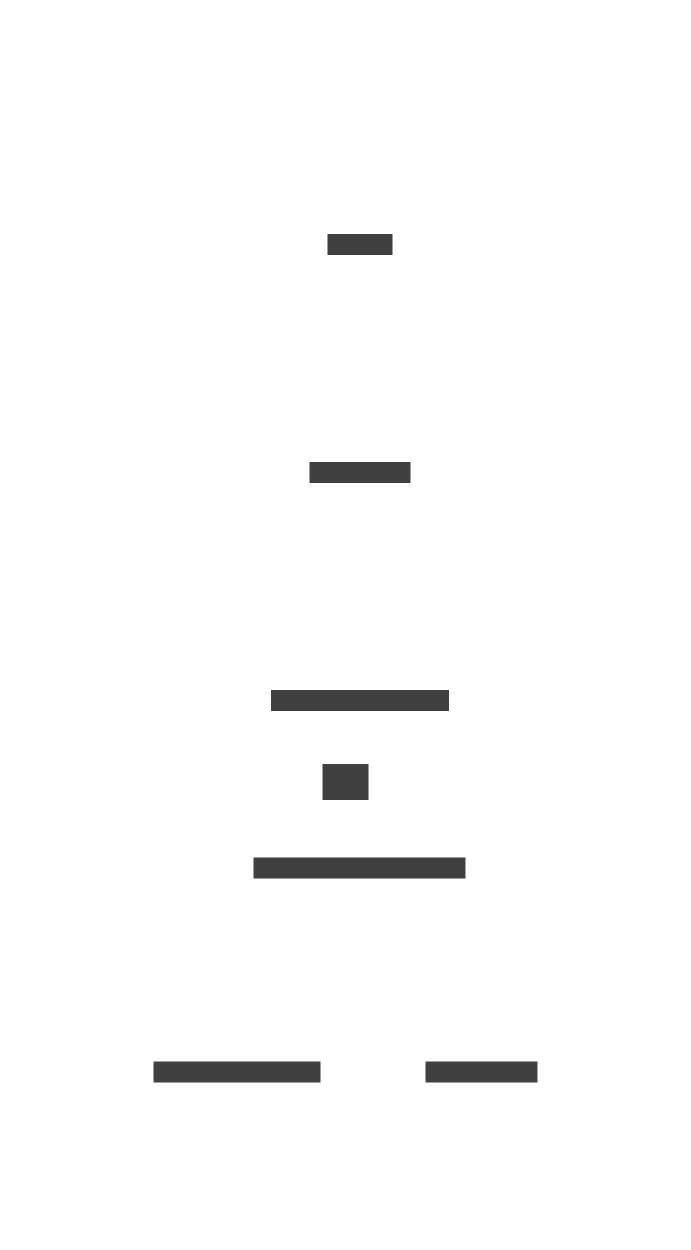
\includegraphics[width=.9\linewidth]{./architecture.png}
\caption{Архитектура CMS}
\end{figure}

\section{Примеры CMS}
\label{sec:orgc4de6eb}

\begin{itemize}
\item Wordpress
\item Joomla
\item Open Cart
\item Drupal
\item 1с-битрикс
\end{itemize}
\end{document}